% Shared content and layout for the four standalone CV entry points.
\usepackage[a4paper,margin=11mm,top=9mm,bottom=10mm]{geometry}
\usepackage[utf8]{inputenc}
\usepackage[T1]{fontenc}
\usepackage[scaled=0.96]{helvet}
\renewcommand{\familydefault}{\sfdefault}
\usepackage{newunicodechar}
\newunicodechar{’}{\textquoteright}
\newunicodechar{·}{\textperiodcentered}
\newunicodechar{œ}{\oe}
\usepackage{graphicx}
\usepackage{xcolor}
\usepackage{hyperref}
\usepackage{xurl}
\usepackage{enumitem}
\usepackage{tabularx}
\usepackage{needspace}
\usepackage{etoolbox}
\usepackage{microtype}

\definecolor{cvnavy}{HTML}{17365D}
\definecolor{cvslate}{HTML}{64748B}
\definecolor{cvsoft}{HTML}{CBD5E1}
\definecolor{cvcharcoal}{HTML}{1F2937}
\hypersetup{colorlinks=true,urlcolor=cvcharcoal}
\urlstyle{same}
\pagestyle{empty}
\flushbottom
\setlength{\parindent}{0pt}
\setlength{\parskip}{0pt}
\setlength{\tabcolsep}{0pt}
\setlist[itemize]{leftmargin=11pt,itemsep=1pt,topsep=2pt,parsep=0pt,partopsep=0pt}

\newcommand{\Bi}[2]{\ifdefstring{\cvlang}{en}{#1}{#2}}
\newcommand{\ContactSep}{\textcolor{cvsoft}{|}}
\newcommand{\Section}[1]{%
  \Needspace{2.5\baselineskip}%
  \vspace{3pt plus 1fil}%
  \noindent{\color{cvnavy}\bfseries\fontsize{12}{13.5}\selectfont #1}\par
  \vspace{1.5pt}{\color{cvslate}\hrule height 0.55pt}\vspace{1.5pt plus 1pt}%
}
\newcommand{\Entry}[2]{%
  \Needspace{2\baselineskip}%
  \begin{tabularx}{\linewidth}{@{}Xr@{}}
    {\color{cvcharcoal}\bfseries\fontsize{10.5}{11.8}\selectfont #1} &
    {\color{cvslate}\fontsize{9.2}{10.5}\selectfont #2}
  \end{tabularx}\par\vspace{-1pt}%
}
\newcommand{\Detail}[1]{{\color{cvslate}#1}\par}
\newcommand{\Skill}[2]{\textbf{#1:} #2\par}
\newcommand{\Project}[4]{%
  \Entry{#1}{#2}%
  #3\par
  \Skill{\Bi{Technologies}{Technologies}}{#4}\vspace{2pt}%
}
\newcommand{\Header}[1]{%
  \ifdefstring{\cvstyle}{visual}{%
    \noindent
    \begin{minipage}{\linewidth}
      \makebox[0pt][l]{%
        \raisebox{-17mm}[17mm][0pt]{%
          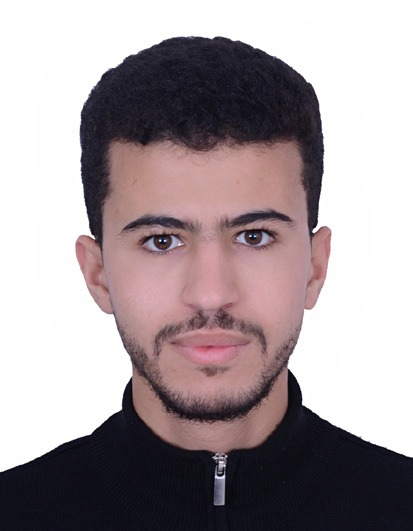
\includegraphics[width=36mm,height=46mm,keepaspectratio]{public/images/oualid-ait-alla.jpg}%
        }%
      }%
      \begin{minipage}{\linewidth}
        \centering
        {\color{cvnavy}\fontsize{23}{25}\selectfont\bfseries AIT ALLA Oualid}\par
        \vspace{1pt}
        {\fontsize{12}{13.5}\selectfont\bfseries
          \Bi{AI Engineer | Machine Learning Engineer | Data Scientist}
             {Ingénieur IA | Ingénieur Machine Learning | Data Scientist}\par}
        \vspace{1pt}
        {\fontsize{9}{10.5}\selectfont
          \Bi{Seeking an Internship | AI Engineering, Data Science \& Cybersecurity}
             {À la recherche d’un stage | Ingénierie IA, Data Science \& Cybersécurité}\par}
        \vspace{2pt}
        {\color{cvcharcoal}\fontsize{8.8}{10}\selectfont
          \Bi{Beni Mellal, Morocco}{Beni Mellal, Maroc}
          \quad\ContactSep\quad \href{mailto:oualidaitalla18@gmail.com}{oualidaitalla18@gmail.com}
          \quad\ContactSep\quad +212 609 831 277\par}
        \makebox[\linewidth][l]{%
          \hspace*{42mm}%
          \makebox[\dimexpr\linewidth-42mm\relax][c]{%
            \color{cvcharcoal}\fontsize{7.5}{8.8}\selectfont
            \url{https://oualid-ait-alla.vercel.app}
            \quad\ContactSep\quad \url{https://www.linkedin.com/in/aitalla-oualid-9797132bb/}
            \quad\ContactSep\quad \url{https://github.com/gimuser}%
          }%
        }\par
      \end{minipage}
    \end{minipage}\par
    \vspace{20pt}
  }{%
    \begin{center}
      {\color{cvnavy}\fontsize{23}{25}\selectfont\bfseries AIT ALLA Oualid\par}
      \vspace{1pt}
      {\fontsize{12}{13.5}\selectfont\bfseries
        \Bi{AI Engineer | Machine Learning Engineer | Data Scientist}
           {Ingénieur IA | Ingénieur Machine Learning | Data Scientist}\par}
      \vspace{1pt}
      {\fontsize{9}{10.5}\selectfont
        \Bi{Seeking an Internship | AI Engineering, Data Science \& Cybersecurity}
           {À la recherche d’un stage | Ingénierie IA, Data Science \& Cybersécurité}\par}
      \vspace{2pt}
      {\color{cvcharcoal}\fontsize{8.8}{10}\selectfont
        \Bi{Beni Mellal, Morocco}{Beni Mellal, Maroc}
        \quad\ContactSep\quad \href{mailto:oualidaitalla18@gmail.com}{oualidaitalla18@gmail.com}
        \quad\ContactSep\quad +212 609 831 277\par}
      {\color{cvcharcoal}\fontsize{8.6}{9.8}\selectfont
        \url{https://oualid-ait-alla.vercel.app}
        \quad\ContactSep\quad \url{https://www.linkedin.com/in/aitalla-oualid-9797132bb/}
        \quad\ContactSep\quad \url{https://github.com/gimuser}\par}
    \end{center}
    \vspace{2pt}
  }%
}
\newcommand{\CVPage}[2]{%
  \begingroup
  \def\cvlang{#1}%
  \def\cvstyle{#2}%
  \color{cvcharcoal}\fontsize{9.8}{11.5}\selectfont
  \setlength{\parskip}{0.7pt}%
  \Header{}%

  \Section{\Bi{Professional Summary}{Profil professionnel}}
  \Bi{Master's student in the final year of Data Science and Information Systems Security at Sultan Moulay Slimane University. Completed a two-month AI Engineering internship at SPORTScore SAS, working on LLM-based document processing, structured-output validation and model quantization. Practical experience in machine learning, generative AI, RAG and reinforcement learning.}
     {Étudiant en dernière année de Master Data Science et Sécurité des Systèmes d’Information à l’Université Sultan Moulay Slimane. A effectué un stage de deux mois en ingénierie IA chez SPORTScore SAS, portant sur le traitement de documents avec des LLM, la validation des sorties structurées et la quantification de modèles. Expérience pratique en Machine Learning, IA générative, RAG et apprentissage par renforcement.}\par

  \Section{\Bi{Technical Skills}{Compétences techniques}}
  \Skill{\Bi{Generative AI}{IA générative}}
    {\Bi{LLMs, RAG, prompt engineering, embeddings, OCR, document processing, JSON Schema, model quantization}
        {LLM, RAG, prompt engineering, embeddings, OCR, traitement documentaire, JSON Schema, quantification de modèles}}
  \Skill{Machine Learning}
    {\Bi{Machine Learning, Deep Learning, Reinforcement Learning (DQN, DDQN), feature engineering, model evaluation, TensorFlow, PyTorch, Scikit-learn}
        {Machine Learning, Deep Learning, apprentissage par renforcement (DQN, DDQN), feature engineering, évaluation de modèles, TensorFlow, PyTorch, Scikit-learn}}
  \Skill{Data Science}
    {\Bi{Python, Pandas, NumPy, data analysis, regression, Power BI, SPSS}
        {Python, Pandas, NumPy, analyse de données, régression, Power BI, SPSS}}
  \Skill{\Bi{Databases}{Bases de données}}{SQL, NoSQL, MongoDB}
  \Skill{\Bi{Cybersecurity}{Cybersécurité}}
    {\Bi{Network security, web application security, cryptography, IDS/IPS, Burp Suite, Kali Linux, Metasploit}
        {Sécurité réseau, sécurité des applications web, cryptographie, IDS/IPS, Burp Suite, Kali Linux, Metasploit}}

  \Section{\Bi{Professional Experience}{Expérience professionnelle}}
  \Entry{\Bi{AI Engineering Intern}{Stagiaire ingénieur en intelligence artificielle}}
    {\Bi{Aug 2026 -- Oct 2026}{Août 2026 -- Oct. 2026}}
  \Detail{\textbf{SPORTScore SAS} \quad|\quad Paris, France}
  \begin{itemize}
    \item \Bi{Contributed to a document-retrieval workflow combining OCR, parsing and vector indexing.}
            {Contribution à un workflow de recherche documentaire combinant OCR, parsing et indexation vectorielle.}
    \item \Bi{Implemented structured-output validation using JSON Schema and constrained generation.}
            {Mise en œuvre de la validation des sorties structurées avec JSON Schema et génération contrainte.}
    \item \Bi{Applied model quantization to improve LLM inference efficiency.}
            {Application de la quantification des modèles pour améliorer l’efficacité de l’inférence LLM.}
    \item \Bi{Evaluated pipeline outputs and documented results with the AI team.}
            {Évaluation des sorties du pipeline et documentation des résultats avec l’équipe IA.}
  \end{itemize}

  \Section{\Bi{Education}{Formation}}
  \Entry{\Bi{Master’s Degree in Data Science and Information Systems Security (in progress)}
             {Master Data Science et Sécurité des Systèmes d’Information (en cours)}}
    {\Bi{Sep 2025 -- Jul 2027 (expected)}{Sept. 2025 -- Juil. 2027 (prévu)}}
  \Detail{\Bi{Sultan Moulay Slimane University, Polydisciplinary Faculty of Beni Mellal}
             {Université Sultan Moulay Slimane, Faculté Polydisciplinaire de Béni Mellal}}
  \Bi{Focus: data science, artificial intelligence, cybersecurity, and secure information systems.}
     {Axes : data science, intelligence artificielle, cybersécurité et systèmes d’information sécurisés.}\par
  \vspace{2.5pt}
  \Entry{\Bi{Bachelor’s Degree in Data Science and Information Systems Security}
             {Licence en Data Science et Sécurité des Systèmes d’Information}}{2025}
  \Detail{\Bi{Sultan Moulay Slimane University, Polydisciplinary Faculty of Beni Mellal}
             {Université Sultan Moulay Slimane, Faculté Polydisciplinaire de Beni Mellal}}
  \Bi{Relevant Coursework: Machine Learning · Feature Engineering · IoT · Information Systems Auditing · Cybersecurity · Python for Data Science.}
     {Matières principales : Machine Learning · Feature Engineering · IoT · Audit des systèmes d’information · Cybersécurité · Python pour la Data Science.}\par
  \vspace{2.5pt}
  \Entry{\Bi{DEUG in Mathematics and Computer Science}{DEUG en Mathématiques et Informatique}}{2024}
  \Detail{\Bi{Sultan Moulay Slimane University, Polydisciplinary Faculty of Beni Mellal}
             {Université Sultan Moulay Slimane, Faculté Polydisciplinaire de Béni Mellal}}
  \Bi{Relevant Coursework: Programming · Algorithms · Data Structures · Probability \& Statistics · Operating Systems.}
     {Matières principales : Programmation · Algorithmique · Structures de données · Probabilités \& Statistiques · Systèmes d’exploitation.}\par

  \Section{\Bi{Professional Projects}{Projets professionnels}}
  \Project{\Bi{SOAR RL Agent}{Agent RL pour SOAR}}{2026}
    {\Bi{Collaborative reinforcement-learning project for security-alert triage in a simulated SOC: FastAPI backend, RL environment, reward system, DQN and DDQN agents, automated tests.}
        {Projet collaboratif d’apprentissage par renforcement pour le triage des alertes dans un SOC simulé : backend FastAPI, environnement RL, système de récompenses, agents DQN et DDQN, tests automatisés.}}
    {Python, FastAPI, Reinforcement Learning, DQN, DDQN, SOAR, Docker Compose}
  \Project{BachelorAI Tutor}{2026}
    {\Bi{RAG-based educational assistant providing answers grounded in academic course materials.}
        {Assistant pédagogique basé sur RAG, fournissant des réponses fondées sur les supports de cours.}}
    {Python, MongoDB, Ollama, RAG}
  \Project{Islamic AI Chat}{2026}
    {\Bi{AI chat application providing answers grounded in trusted Islamic references, with authentication and prompt-injection checks.}
        {Application de chat IA fournissant des réponses fondées sur des références islamiques fiables, avec authentification et protection contre l’injection de prompt.}}
    {MongoDB, LLMs, JWT}

  \Section{\Bi{Soft Skills}{Qualités professionnelles}}
  \Bi{Analytical Thinking · Problem-Solving · Autonomy \& Initiative · Rigor \& Attention to Detail · Professionalism · Commitment \& Diligence}
     {Esprit d’analyse · Résolution de problèmes · Autonomie et esprit d’initiative · Rigueur et attention aux détails · Professionnalisme · Engagement et assiduité}\par

  \Section{\Bi{Languages}{Langues}}
  \Bi{Arabic: Native \quad|\quad English: B2 \quad|\quad French: B2 \quad|\quad Spanish: Beginner}
     {Arabe : langue maternelle \quad|\quad Anglais : B2 \quad|\quad Français : B2 \quad|\quad Espagnol : Débutant}
  \endgroup
}
